%%%%%%%%%%%%%%%%%%%%%%%%%%%%%%%%%%%%%%%%%%%%%%%%%%%%%%%%%%%%%%%%%%%%%%%%%%%%
% AGUtmpl.tex: this template file is for articles formatted with LaTeX2e,
% Modified March 2013
%
% This template includes commands and instructions
% given in the order necessary to produce a final output that will
% satisfy AGU requirements.
%
% PLEASE DO NOT USE YOUR OWN MACROS
% DO NOT USE \newcommand, \renewcommand, or \def.
%
% FOR FIGURES, DO NOT USE \psfrag or \subfigure.
%
%%%%%%%%%%%%%%%%%%%%%%%%%%%%%%%%%%%%%%%%%%%%%%%%%%%%%%%%%%%%%%%%%%%%%%%%%%%%
%
% All questions should be e-mailed to latex@agu.org.
%
%%%%%%%%%%%%%%%%%%%%%%%%%%%%%%%%%%%%%%%%%%%%%%%%%%%%%%%%%%%%%%%%%%%%%%%%%%%%
%
% Step 1: Set the \documentclass
%
% There are two options for article format: two column (default)
% and draft.
%
% PLEASE USE THE DRAFT OPTION TO SUBMIT YOUR PAPERS.
% The draft option produces double spaced output.
%
% Choose the journal abbreviation for the journal you are
% submitting to:

% jgrga JOURNAL OF GEOPHYSICAL RESEARCH
% gbc   GLOBAL BIOCHEMICAL CYCLES
% grl   GEOPHYSICAL RESEARCH LETTERS
% pal   PALEOCEANOGRAPHY
% ras   RADIO SCIENCE
% rog   REVIEWS OF GEOPHYSICS
% tec   TECTONICS
% wrr   WATER RESOURCES RESEARCH
% gc    GEOCHEMISTRY, GEOPHYSICS, GEOSYSTEMS
% sw    SPACE WEATHER
% ms    JAMES
%
%
%
% (If you are submitting to a journal other than jgrga,
% substitute the initials of the journal for "jgrga" below.)

\documentclass[grl]{AGUTeX}

% To create numbered lines:

% If you don't already have lineno.sty, you can download it from
% http://www.ctan.org/tex-archive/macros/latex/contrib/ednotes/
% (or search the internet for lineno.sty ctan), available at TeX Archive Network (CTAN).
% Take care that you always use the latest version.

% To activate the commands, uncomment \usepackage{lineno}
% and \linenumbers*[1]command, below:

%\usepackage{lineno}
%\linenumbers*[1]

%  To add line numbers to lines with equations:
%  \begin{linenomath*}
%  \begin{equation}
%  \end{equation}
%  \end{linenomath*}
%%%%%%%%%%%%%%%%%%%%%%%%%%%%%%%%%%%%%%%%%%%%%%%%%%%%%%%%%%%%%%%%%%%%%%%%%
% Figures and Tables
%
%
% DO NOT USE \psfrag or \subfigure commands.
%
%  Figures and tables should be placed AT THE END OF THE ARTICLE,
%  after the references.
%
%  Uncomment the following command to include .eps files
%  (comment out this line for draft format):
\usepackage{graphicx}
%
%  Uncomment the following command to allow illustrations to print
%   when using Draft:
\setkeys{Gin}{draft=false}
%
% Substitute one of the following for [dvips] above
% if you are using a different driver program and want to
% proof your illustrations on your machine:
%
% [xdvi], [dvipdf], [dvipsone], [dviwindo], [emtex], [dviwin],
% [pctexps],  [pctexwin],  [pctexh p],  [pctex32], [truetex], [tcidvi],
% [oztex], [textures]
%
% See how to enter figures and tables at the end of the article, after
% references.
%
%% ------------------------------------------------------------------------ %%
%
%  ENTER PREAMBLE
%
%% ------------------------------------------------------------------------ %%

% Author names in capital letters:
\authorrunninghead{ZHANG ET AL.}

% Shorter version of title entered in capital letters:
\titlerunninghead{Parallelization of nonlocal operator for GPS RO data}

%Corresponding author mailing address and e-mail address:
\authoraddr{Corresponding author: Dr. Xin Zhang,
Mesoscale and Microscale Meteorology Division, 
National Center for Atmospheric Research, Boulder, CO 80307-3000, USA.
(xinzhang@ucar.edu)}

\begin{document}

%% ------------------------------------------------------------------------ %%
%
%  TITLE
%
%% ------------------------------------------------------------------------ %%


\title{Strategies for parallel data assimilation of GPS radio occultation data with a nonlocal observation operator}
%
% e.g., \title{Terrestrial ring current:
% Origin, formation, and decay $\alpha\beta\Gamma\Delta$}
%

%% ------------------------------------------------------------------------ %%
%
%  AUTHORS AND AFFILIATIONS
%
%% ------------------------------------------------------------------------ %%


%Use \author{\altaffilmark{}} and \altaffiltext{}

% \altaffilmark will produce footnote;
% matching \altaffiltext will appear at bottom of page.

\authors{Xin Zhang,\altaffilmark{1}
 Shu-Ya Chen,\altaffilmark{1} Ying-Hwa Kuo,\altaffilmark{1}
 , and Xiang-Yu Huang\altaffilmark{1}}

\altaffiltext{1}{Mesoscale and Microscale Meteorology Division, 
National Center for Atmospheric Research, Boulder, CO 80307-3000, USA.}

%\altaffiltext{2}{Department of Geography, Ohio State University,
%Columbus, Ohio, USA.}

%\altaffiltext{3}{Department of Space Sciences, University of
%Michigan, Ann Arbor, Michigan, USA.}

%\altaffiltext{4}{Division of Hydrologic Sciences, Desert Research
%Institute, Reno, Nevada, USA.}

%\altaffiltext{5}{Dipartimento di Idraulica, Trasporti ed
%Infrastrutture Civili, Politecnico di Torino, Turin, Italy.}

%% ------------------------------------------------------------------------ %%
%
%  ABSTRACT
%
%% ------------------------------------------------------------------------ %%

% >> Do NOT include any \begin...\end commands within
% >> the body of the abstract.

\begin{abstract}
Several parallel strategies are designed and implemented in WRF data assimilation system to demonstrate the parallel assimilation techniques the GPS radio occultation (RO) sounding with the nonlocal excess phase delay operator, which is computational expensive and has been proven to produce significant better analysis for numerical weather predictions compared to local refractivity operator. Due to the uneven geographic distribution of the observations, for parallel models adopting domain-decomposition approach, the round-robin scheduling is adopted to distribute GPS RO observations among the processing cores to balance the workload among the processing cores. The wallclock time required to complete $5$ iterations of minimization on the demonstrated Antarctic with $106$ GPS RO observations, is reduced from more than $3.5$ hours with single processor to $2.5$ minutes with $106$ processing cores. These strategies present the possibility of the application of the nonlocal GPS excess phase operator in operational data assimilation systems with a cut-off time limit.
\end{abstract}

%% ------------------------------------------------------------------------ %%
%
%  BEGIN ARTICLE
%
%% ------------------------------------------------------------------------ %%

% The body of the article must start with a \begin{article} command
%
% \end{article} must follow the references section, before the figures
%  and tables.

\begin{article}

%% ------------------------------------------------------------------------ %%
%
%  TEXT
%
%% ------------------------------------------------------------------------ %%

\section{Introduction}
The observations from the global positioning system (GPS) radio occultation (RO) limb sounding technique has been proven as a valuable observation of atmosphere for numerical weather prediction (NWP) and climate research. Compared to conventional radiosonde sounding, GPS RO data has several advantages such ad a high vertical resolution, no need for calibration, unaffected by cloud cover and rainfall, and global coverage. In Particular, in the middle of upper troposphere, the GPS RO measurements have accuracy comparable with or better than that of radiosondes (\citet{Kuo2005}). Since the launch of the Constellation Observing System for Meteorology, Ionosphere, and Climate (COSMIC) mission in 2006, approximately ${\sim}$1500-2500 globally distributed GPS RO sounding are provided per day in near-real time. The assimilation of GPS RO occultation sounding data into global (NWP) systems has been shown to significantly improve weather forecast skill. There are several reasons for this, including the unbiased nature of the RO measurements, the high vertical resolution of the soundings, and the fact that the technique is almost insensitive to aerosols, clouds and precipitation. The COSMIC GPS RO sounding are currently being used at several global operational NWP centers, including the National Centers for Environmental Prediction (NCEP; \citet{Cucurull2008}), the European Centre for Medium-Range Weather Forecasts (ECMWF; \citet{Healy2008}), the Met Office (UKMO), and M\'et\'eo France (\citet{Poli2009}).

Due to the success of COSMIC, U.S. agencies and Taiwan have decided to move forward with a follow-on RO mission (called FORMOSAT-7/COSMIC-2) that will launch six satellites into low-inclination orbits in late 2015, and another six satellites into high-inclination orbits in early 2018. The COSMIC-2 mission will provide nearly an order of magnitude more RO data increase in the number of atmospheric and ionospheric observations that will greatly benefit the research and operational communities (http://www.cosmic.ucar.edu/cosmic2/).

Because both the local and nonlocal operators had been implemented in the WRF data assimilation system (WRFDA, \citet{Barker2012}), the 3D-Var approach in WRFDA will be used throughout this paper to demonstrate the parallelization of GPS nonlocal operator. We believe that the parallel strategies for nonlocal operator are general and applicable for any parallel data assimilation systems (include 3D-Var, 4D-Var, and Ensemble Kalman Filter) employing the domain-decomposition method.


%%%%%%%%%%%%%%%%%%%%%%%%%%%%%%%%%%%%%%%%%%%%%%%%%%
\section{Local and nonlocal GPS RO Operators}
In both local and nonlocal GPS RO operators, the neutral atmospheric refractivity can be calculated from model variables via the following relationship
\begin{equation}
\label{ref}
N = 77.6\frac{P}{T} + 3.73\times10^5\frac{P Q}{T^2(0.622+0.378Q)}
\end{equation}
where $P$ is the total atmospheric pressure in $hPa$; $T$ is the atmospheric temperature in $K$; and $Q$ is the specific humidity in ${kg}/{kg}$. The local GPS RO refractivity operator assumes that the observed refractivity is modeled as the local refractivity at the perigee point where the GPS ray is closest to the earth. The first guess fields of $P$, $T$ and $Q$ are interpolated horizontally and vertically to the perigee point of the RO observation and the Eqs. (\ref{ref}) is used to calculate the local refractivity. The local GPS RO refractivity operator is simple and low computational cost, and it is used by most of the data assimilation systems. 

To account for the variations of the atmospheric states along the GPS ray paths, the nonlocal excess phase operator, introduced by \citet{Soko2005}, simulates the excess phase by integrating the local refractivity along the ray path, which is approximated by a straight line. The new observable (excess phase) is defined as
 \begin{equation}
 \label{excess}
 S = \int_{ray} N\; \mathrm{d}l
  \end{equation}
  where $l$ is the ray path. There are two steps associated with the implementation of the nonlocal operator (\citet{ChenSY}, \citet{Ma2009}, and \citet{Liu2008}): Firstly, the observed excess phase is calculated by integrating the refractivity from RO observations:
  \begin{equation}
  \label{excess-o}
  S_{obs} = \int_{ray} N_{RO}(r)\; \mathrm{d}l
  \end{equation}
  where $r$ is the radius vector derived from $r=r_c+z$, $r_c$ is the local curvature radius of the earth, and $z$ is the height above the earth's surface, $N_{RO}$ is the observed refractivity interpolated on the model mean heights of the tangent point position by a vertical average. The next step is to calculate the model counterpart $S_{mod}$, which is given by
 \begin{equation}
 \label{excess-m}
 S_{mod} = \int_{ray} N_{mod}(r)\; \mathrm{d}l
 \end{equation}
where  $N_{mod}$ is the simulated refractivity from first guess fields of $T$, $P$, and $Q$  and interpolated at the tangent point position. 

Compared to the local GPS refractivity operator, the computational cost of the nonlocal excess phase operator is increased dramatically due to the integration of refractivity along the GPS ray. \citet{Liu2008} reports that the cost of nonlocal to local operator is at least $100$ times on a Linux cluster of NCAR. To justify the necessity to parallel the GPS RO nonlocal operator, an Antarctic domain with $30km$ horizontal resolution, shown as Fig. \ref{domain}, is chosen to demonstrate the computational cost of GPS RO operators. This is a WRF ARW model domain of 1800 UTC 11 December 2007 with $401\times401$ mesh size and 55 vertical layers between surface and $10$ $hPa$. Fig. \ref{domain} also shows the locations of the $106$ GPS RO profiles within $\pm3$ hours window centered at 1800UTC. The $106$ GPS RO profiles are assimilated with WRFDA 3D-Var on NCAR's super computer yellowstone (http://www2.cisl.ucar.edu/resources/yellowstone) and the wallclock time of only 5 iterations of minimization are recorded to demonstrate the computational costs. After excluding the program initialization and I/O, with single processing core, It takes only $146s$ to assimilate $106$ GPS RO profiles by local operator. However, about $12,762s$ are needed to run 5 iterations with nonlocal operator. The ratio of the computational cost of nonlocal to local operator is about 87 for this case. Note that the cost of nonlocal operator depends on the domain coverage, model top and the vertical model levels. In terms of the production 3D-Var run with 60 iterations (2 outer loops) approximately, the wallclock time for this case will be more than 42 hours on yellowstone. Therefore, the cost of nonlocal operator with single processing core is extremely unaffordable for both research and operational purposes.

%%%%%%%%%%%%%%%%%%%%%%%%%%%%%%%%%%%%%%%%%%%%%%%%%%
\section{Parallelization strategy}
\label{strategy}
Most of the atmospheric models employ the horizontal domain-decomposition method for parallel processing. Their data assimilation systems usually use the same homogeneous data distribution method for observation processing and assimilation. The observations will be distributed geographically in connected domains and with no redistribution. The drawback is the lack of load balance. Most of the observation operators for conventional data are simple and cheap, the performance of this method is still desirable. However, for satellite radiance data assimilation, due to the involvement of radiative transfer model, the radiance operator is expensive and load unbalance issue has to be considered for operational practice. We may either change the way of the horizontal domain-decomposition method to have each subdomain cover similar number of radiance data, or redistribute the radiance data among processing cores to have each core has similar workload. Please note that the load balance algorithm might be costly and complicated. The observation operator in data assimilation represents the physical transform or projection from model variables space to observation space, as well as the spatial and/or temporal interpolations. In current operational data assimilation systems, the physical transforms in almost all observation operators are computed locally or column-wisely in terms of the model space. This is why the horizontal domain-decomposition method is still chosen for the observational data distribution. 

The difficulty of the nonlocal operator parallelization with current data partition approach roots in the nonlocal integral nature of Eq. (\ref{excess-m}) along the ray-paths at all vertical levels above the tangent point and below the model top. The ray-path might intercepts several subdomains located on different processing cores respectively and each processing core is only aware of the atmospheric states of the local subdomain. Apparently, the most suitable strategy to parallel nonlocal GPS RO operator is the ray-path-wise distribution among processing cores (\citet{Zhang2004}), which means that the distribution of the workload among processing cores is based on the number of the GPS ray-paths, not on the geographic location of the observations. However, in our parallelization strategy, we must consider the existed data partitioning approach to minimize the implementation cost. 

Although Eq. (\ref{excess-m}) is the integration of the refractivity along the ray-path, which might not be calculated locally, we noticed that only one derived variable ($N_{mod}$) is used for the integration. The calculate of model simulated refractivity-- $N_{mod}$ from fist guess fields with Eq. (\ref{ref}) is trivial and each processing core can calculate the grid-point-wise $N_{mod}$  of subdomain locally in advance. Next, the parallel collecting-and-broadcasting operation collects the local $N_{mod}$ from each subdomain to a global $N_{mod}$ and broadcasts the global $N_{mod}$ to each processing core. Therefore, each processing core (subdomain) is aware of the simulated refractivity globally and the integration is able to be done on the whole ray-path.

The cost for this parallel strategy is the memory usage increasing. In this case, there will be about $67MB$ additional memory being allocated for the global model refractivity on each processing core. ($401\times401\times55\times8=70,752,440$ $Bytes$ with double precision). For variational data assimilation approaches, a global model refractivity increment array and a global model refractivity adjoint array are needed for the tangent linear and adjoint nonlocal operators, respectively. For modern distributed memory super computers, the additional several hundreds megabytes memory requirement per processing core is affordable in general. However, cautions have to be taken with multi-core computer nodes that the total memory requirements for each precessing core should not exceed the hard-wired memory size.

With the implementation of above parallel strategy (experiment "Parallel") , Fig. \ref{timing}(a) shows the parallel wallclock timing results with up to 512 processing cores on NCAR's yellowstone (red bars represent experiment "Parallel"). The wallclock time of 5 iterations minimization reduced from around $3.5$ hours with serial run to $279$ seconds with 512 processing cores. 

%%%%%%%%%%%%%%%%%%%%%%%%%%%%%%%%%%%%%%%%%%%%%%%%%%
\section{Load balance}
Fig. \ref{spd} shows the parallel speedups, which are the ratio of the wallclock times of parallel runs against that of the serial run. The black line is the linear parallel speedup and represents the ideal speedup or acceleration when multiple processing cores are used. The red line represents experiment "Parallel". The speedup with $512$ processing cores is $46$ and one may argue that  the actual speedup is much lower than the ideal speedup ($512$) and the parallelization strategy is not cost-effective. Therefore, the analysis of the parallel algorithm of the GPS RO operator will be helpful to understand the unsatisfactory speedup and identify the reason behind.

In Sec. \ref{strategy}, we emphasized that we have to consider the existed horizontal domain-decomposition method for the GPS RO data distribution, which indicates that each GPS RO profile is assigned to the connected domain based on its geographic location, and moreover, it is known that the nonlocal excess phase operator for GPS RO data is expensive and dominates the computational cost in this case. The locations of the GPS RO profiles are not fixed and changes for every occultation. The geographic distribution of GPS RO profiles is not even  (see Fig. \ref{domain}), It is very likely that some processing cores or domains get more GPS RO profiles than others, which leads to the fact that the overall performance is solely determined by the workload of the processing cores which being assigned the most number of profiles to process. Fig. \ref{timing}(b) shows the variation of the maximum number of assigned observations per subdomain with the numbers of processing cores (red bars represent experiment "Parallel"). Because the uneven geographic distribution of the GPS RO profiles, even we used $512$ processing cores, there is still one out of $512$ subdomains covers two GPS RO profiles. Therefore, the theoretic speedup with $512$ processing cores is $106/2=53$ and the actual speedup of $46$ should be considered as efficient enough. It is impossible to achieve the ideal speedup before solving the load unbalance issue. Visual comparison of (a) and (b) in Fig. \ref{timing} suggests that the parallel performance has a very high correlation with the maximum number of the observation per processing core/subdomain and the load unbalance is the bottleneck of the overall parallel performance.

We have indicated that the most suitable parallel strategy for the nonlocal GPS RO operator is the ray-path-wise distribution. Taking advantage of the parallel strategy implemented in Sec. \ref{strategy}, each processing core is aware of the global simulated model refractivity, which enables each processing core to calculate the integral of Eq. \ref{excess-m} along any ray-path. Therefore, it is feasible to distribute the GPS RO data ray-by-ray among processing cores in a round-robin fashion. However, taking into account the cost of implmemtation, it is much easier to distribute the GPS RO data profile-by-profile among processing cores in terms of the amount of code modification. Since different GPS RO profile may includes different number of GPS ray-paths at vertical levels above the tangent point and below the model top, the profile-by-profile distribution may sacrifice some of the load balance compared to the ray-by-ray distribution. 

The experiment "Loadbalance" in Fig. \ref{timing}(a) shows the wallclock time spent with the number of processing cores up to $128$. Actually, $106$ is the minimum number of processing cores for this case to get the maximum theoretic parallel efficiency since we have $106$ GPS RO profiles.  With the round-robin distribution of the GPS RO profiles, each processing core is assigned with one profile. We also ran the case with $106$, $256$, and $512$ processing cores, respectively, and got the same or similar timing results as that of $128$ processing cores. With $128$ processing cores, the wallclock time is reduced to $162$ seconds for 5 iterations minimization including initialization and I/O. Compared to $492$ seconds with $128$ processing cores and $279$ seconds with $512$ processing cores in Sec. \ref{strategy}, the load balance strategy tremendously increases the parallel efficiency of the nonlocal excess phase GPS RO operator. The experiment "Loadbalance" in Fig. \ref{spd} shows that the speedup with $128$ processing cores is $80$. More precisely speaking, the speedup with $106$ processing core is $80$. Without the load balance strategy, the speedup with $128$ processing cores is $33$. Again, the high correlation between the wallclock times and the maximum number of observations per processing cores of experiment "Loadbalance" in (a) and (b) of Fig. \ref{timing} confirms that the the importance of the load balance strategy in parallel data assimilation of GPS RO data with nonlocal operator.

%%%%%%%%%%%%%%%%%%%%%%%%%%%%%%%%%%%%%%%%%%%%%%%%%%
\section{Optimization on WRFDA }
In variational data assimilation methods, not only the observation operator is needed to calculate the innovation, but also the corresponding tangent linear and adjoint observation operators are required during the minimization. The tangent linear and adjoint operators are used to evolve the perturbations forward and backward along the basic trajectory, respectively. Therefore, it is an economic way to save the computational cost if the basic trajectory could be recorded, other than recomputed, during the calculation of the innovation. In terms of the nonlocal GPS RO operator implementation in the WRFDA system (\citet{ChenSY}), the locations of each ray-path should be recored during the innovation calculation and the recorded location information of each ray-path will be used in tangent linear adjoint operators directly. The experiment "Optimization" in Fig. \ref{timing}(a) shows the wallclock timing results with this further optimization. Averaged $4\% \sim 10\%$ further acceleration is observed.

%%%%%%%%%%%%%%%%%%%%%%%%%%%%%%%%%%%%%%%%%%%%%%%%%%
\section{Summary and discussion}
The nonlocal excess phase operator for GPS RO data has been demonstrated to be a solid and promising method to simulate the the observed GPS excess phase delay from the model states, which is the one of the key component in data assimilation systems. However, due to its computational cost and the nonlocal nature in the algorithm which includes the integration along the GPS ray-path across the model domain, it is not easy to implement this new operator in data assimilation systems parallelized on the 2-D horizontal domain decomposition method. Therefore, it has been tested only in some research configurations with affordable number of observations.

To parallel the nonlocal excess phase GPS RO operator, the first strategy is to enable each processing core to be aware of the global simulated model refractivity, which is the only variable needed for the nonlocal operator and is calculated in advance. Thus, each processing core can process the GPS observations geographically located within its connected domain. However, the performance analysis reveals that the load unbalance associated the default geographic observation distribution among processing cores seriously constrains the parallel efficiency. Leveraging the implementation of the first strategy, GPS RO profiles can be alternatively distributed among processing cores in a round-robin fashion, which ensures the best possible load balance with available computing resource. The demonstration case with $106$ GPS RO profiles over a Antarctic domain shows that the wallclock time for 5 iterations minimization with WRFDA reduced from about 3.5 hours with one processing core to approximately 2.5 minutes with $106$ processing cores. This is affordable in terms of both research and operational practices.

Depends on the height of tangent point of the GPS occultation, different GPS RO profiles may has different number of levels, therefore, different number of ray-paths. As mentioned before, better load balance and further acceleration is still possible if the GPS RO data is distributed among processing cores ray by ray. However, the ray-path has to be determined before the data distribution.


%%% End of body of article:

%%%%%%%%%%%%%%%%%%%%%%%%%%%%%%%%
%% Optional Appendix goes here
%
% \appendix resets counters and redefines section heads
% but doesn't print anything.
% After typing  \appendix
%
% \section{Here Is Appendix Title}
% will show
% Appendix A: Here Is Appendix Title
%
%%%%%%%%%%%%%%%%%%%%%%%%%%%%%%%%%%%%%%%%%%%%%%%%%%%%%%%%%%%%%%%%
%
% Optional Glossary or Notation section, goes here
%
%%%%%%%%%%%%%%
% Glossary is only allowed in Reviews of Geophysics
% \section*{Glossary}
% \paragraph{Term}
% Term Definition here
%
%%%%%%%%%%%%%%
% Notation -- End each entry with a period.
% \begin{notation}
% Term & definition.\\
% Second term & second definition.\\
% \end{notation}
%%%%%%%%%%%%%%%%%%%%%%%%%%%%%%%%%%%%%%%%%%%%%%%%%%%%%%%%%%%%%%%%
%
%  ACKNOWLEDGMENTS

\begin{acknowledgments}
(Text here)
\end{acknowledgments}

%% ------------------------------------------------------------------------ %%
%%  REFERENCE LIST AND TEXT CITATIONS
%
% Either type in your references using
% \begin{thebibliography}{}
% \bibitem{}
% Text
% \end{thebibliography}
%
% Or,
%
% If you use BiBTeX for your references, please use the agufull08.bst file (available at % ftp://ftp.agu.org/journals/latex/journals/Manuscript-Preparation/) to produce your .bbl
% file and copy the contents into your paper here.
%
% Follow these steps:
% 1. Run LaTeX on your LaTeX file.
%
% 2. Make sure the bibliography style appears as \bibliographystyle{agufull08}. Run BiBTeX on your LaTeX
% file.
%
% 3. Open the new .bbl file containing the reference list and
%   copy all the contents into your LaTeX file here.
%
% 4. Comment out the old \bibliographystyle and \bibliography commands.
%
% 5. Run LaTeX on your new file before submitting.
%
% AGU does not want a .bib or a .bbl file. Please copy in the contents of your .bbl file here.

\begin{thebibliography}{}

\providecommand{\natexlab}[1]{#1}
\expandafter\ifx\csname urlstyle\endcsname\relax
  \providecommand{\doi}[1]{doi:\discretionary{}{}{}#1}\else
  \providecommand{\doi}{doi:\discretionary{}{}{}\begingroup
  \urlstyle{rm}\Url}\fi
%
\bibitem[{\textit{Barker et~al.}(2012)}]{Barker2012}
Barker, D., and Coauthors (2012), The Weather Research and Forecasting Model's Community Variational/Ensemble Data Assimilation System: WRFDA. \textit{Bull. Amer. Meteor. Soc.}, \textit{93}, 831�843, \doi{10.1175/BAMS-D-11-00167.1}.
%
\bibitem[{\textit{Chen et~al.}(2009)}]{ChenSY}
Chen, S.~Y., C.~Y. Huang, K.~Y. Kuo, Y.~R. Guo, and S.~Sokolovskiy (2009), Assimilation of GPS refractivity from FORMOSAT-3/COSMIC using a nonlocal operator with WRF 3DVAR and its impact on the prediction of a typhoon event, \textit{Terr. Atmos. Ocean Sci.}, \textit{20}(1), 133--154, \doi{10.3319/TAO.2007.11.29.01(F3C)}.
%
\bibitem[{\textit{Cucurull and Derber}(2008)}]{Cucurull2008}
Cucurull, L., and J.~C. Derber (2008), Operational implementation of COSMIC observations into NCEP�s global data assimilation system. \textit{Wea. Forecasting}, \textit{23}, 702--711.
%
\bibitem[{\textit{Healy}(2008)}]{Healy2008}
Healy, S.~B. (2008), Forecast impact experiment with a constellation of GPS radio occultation receivers. \textit{Atmos. Sci. Lett.}, \textit{9}, 111--118.
%
\bibitem[{\textit{Anderson and Collins}(2007)}]{Anderson2007}
Anderson, J.~L. and N. Collins (2007), Scalable Implementations of Ensemble Filter Algorithms for Data Assimilation. \textit{J. Atmos. Oceanic Technol.}, \textit{24}, 1452--1463, \doi{10.1175/JTECH2049.1}
%
\bibitem[{\textit{Kuo et~al.}(2005)}]{Kuo2005}
Kuo, Y.~H., W.~S. Schreiner, J.~Wang, D.~L. Rossiter, and Y.~Zhang (2005), Comparison of GPS radio occultation soundings with radiosondes. \textit{Geophys. Res. Lett.}, \textit{32}, L05817, \doi{10.1029/2004GL021443}.
%
\bibitem[{\textit{Liu et~al.}(2008)}]{Liu2008}
Liu, H., J.~Anderson, Y.~H. Kuo, C.~Snyder, and A.~Caya (2008), Evaluation of a Nonlocal Quasi-Phase Observation Operator in Assimilation of CHAMP Radio Occultation Refractivity with WRF. \textit{Mon. Wea. Rev.}, \textit{136}, 24--256, \doi{10.1175/2007MWR2042.1}.
%
\bibitem[{\textit{Ma et~al.}(2009)}]{Ma2009}
Ma, Z., Y.~H. Kuo, B.~Wang, W.~S. Wu, and S.~Sokolovskiy (2009), Comparison of Local and Nonlocal Observation Operators for the Assimilation of GPS RO Data with the NCEP GSI System: An OSSE Study. \textit{Mon. Wea. Rev.}, \textit{137}, 3575--3587, \doi{10.1175/2009MWR2809.1}.
%
\bibitem[{\textit{Ma et~al.}(2011)}]{Ma2011}
Ma, Z., Y.~H. Kuo, F.~M. Ralph, P.~J. Neiman, G.~A. Wick, E.~Sukovich, and B.~Wang (2011), Assimilation of GPS Radio Occultation Data for an Intense Atmospheric River with the NCEP Regional GSI System. \textit{Mon. Wea. Rev.}, \textit{139}, 2170--2183, \doi{10.1175/2011MWR3342.1}.
%
\bibitem[{\textit{Poli et~al.}(2009)}]{Poli2009}
Poli, P., P.~Moll, D.~Puech, F.~Rabier, and S.~Healy (2009), Quality control, error analysis and impact assessment of FORMOSAT-3/COSMIC in numerical weather prediction. \textit{Terr. Atmos. Oceanic Sci.}, \textit{20}, 101--113.
%
\bibitem[{\textit{Shao et~al.}(2009)}]{Shao2009}
Shao, H., X.~Zou, and G.~A. Hajj (2009), Test of a non-local excess phase delay operator for GPS radio occultation data assimilation. \textit{J. Appl. Remote Sens.}, \textit{3}, 033508, \doi{10.1117/1.3094060}.
%
\bibitem[{\textit{Sokolovskiy et~al.}(2005a)}]{Soko2005}
Sokolovskiy, S., Y.~H. Kuo, and W.~Wang (2005), Evaluation of a linear phase observation operator with CHAMP radio occultation data and high-resolution regional analysis. \textit{Mon. Wea. Rev.}, \textit{133}, 3053--3059. 
%
\bibitem[{\textit{Zhang et~al.}(2004)}]{Zhang2004}
Zhang X., Y.~Liu, B.~Wang, and Z.~Ji (2004), Parallel computing of a variational data assimilation model for GPS/MET observation using the ray-tracing method. \textit{adv. atmos. sci}, \textit{21}, 220--226, \doi{10.1007/BF02915708}

%
%\bibitem[{\textit{Colton and Kress}(1983)}]{ColtonKress1}
%Colton, D., and R.~Kress (1983), \textit{Integral Equation Methods in
%  Scattering Theory}, John Wiley, New York.
%
%\bibitem[{\textit{Hsiao et~al.}(1991)\textit{Hsiao, Stephan, and
%  Wendland}}]{StephanHsiao}
%Hsiao, G.~C., E.~P. Stephan, and W.~L. Wendland (1991), On the {D}irichlet
%  problem in elasticity for a domain exterior to an arc, \textit{J. Comput.
%  Appl. Math.}, \textit{34}(1), 1--19.
%
%\bibitem[{\textit{Lu and Ando}(2012)}]{LuAndo}
%Lu, P., and M.~Ando (2012), Difference of scattering geometrical optics
%  components and line integrals of currents in modified edge representation,
%  \textit{Radio Sci.}, \textit{47},  RS3007, \doi{10.1029/2011RS004899}.

\end{thebibliography}

%Reference citation examples:

%...as shown by \textit{Kilby} [2008].
%...as shown by {\textit  {Lewin}} [1976], {\textit  {Carson}} [1986], {\textit  {Bartholdy and Billi}} [2002], and {\textit  {Rinaldi}} [2003].
%...has been shown [\textit{Kilby et al.}, 2008].
%...has been shown [{\textit  {Lewin}}, 1976; {\textit  {Carson}}, 1986; {\textit  {Bartholdy and Billi}}, 2002; {\textit  {Rinaldi}}, 2003].
%...has been shown [e.g., {\textit  {Lewin}}, 1976; {\textit  {Carson}}, 1986; {\textit  {Bartholdy and Billi}}, 2002; {\textit  {Rinaldi}}, 2003].

%...as shown by \citet{jskilby}.
%...as shown by \citet{lewin76}, \citet{carson86}, \citet{bartoldy02}, and \citet{rinaldi03}.
%...has been shown \citep{jskilbye}.
%...has been shown \citep{lewin76,carson86,bartoldy02,rinaldi03}.
%...has been shown \citep [e.g.,][]{lewin76,carson86,bartoldy02,rinaldi03}.
%
% Please use ONLY \citet and \citep for reference citations.
% DO NOT use other cite commands (e.g., \cite, \citeyear, \nocite, \citealp, etc.).

%% ------------------------------------------------------------------------ %%
%
%  END ARTICLE
%
%% ------------------------------------------------------------------------ %%
\end{article}
%
%
%% Enter Figures and Tables here:
%
% DO NOT USE \psfrag or \subfigure commands.
%
% Figure captions go below the figure.
% Table titles go above tables; all other caption information
%  should be placed in footnotes below the table.
%
%----------------
% EXAMPLE FIGURE
%
\begin{figure}
\noindent\includegraphics[width=20pc]{figures/obsloc2007121118.eps}
\caption{Experiment domain and the locations of $106$ GPS RO profiles (blue dots) within $\pm3$ hours of 1800 UTC 11 December 2007}
\label{domain}
\end{figure}
%
\begin{figure}
\noindent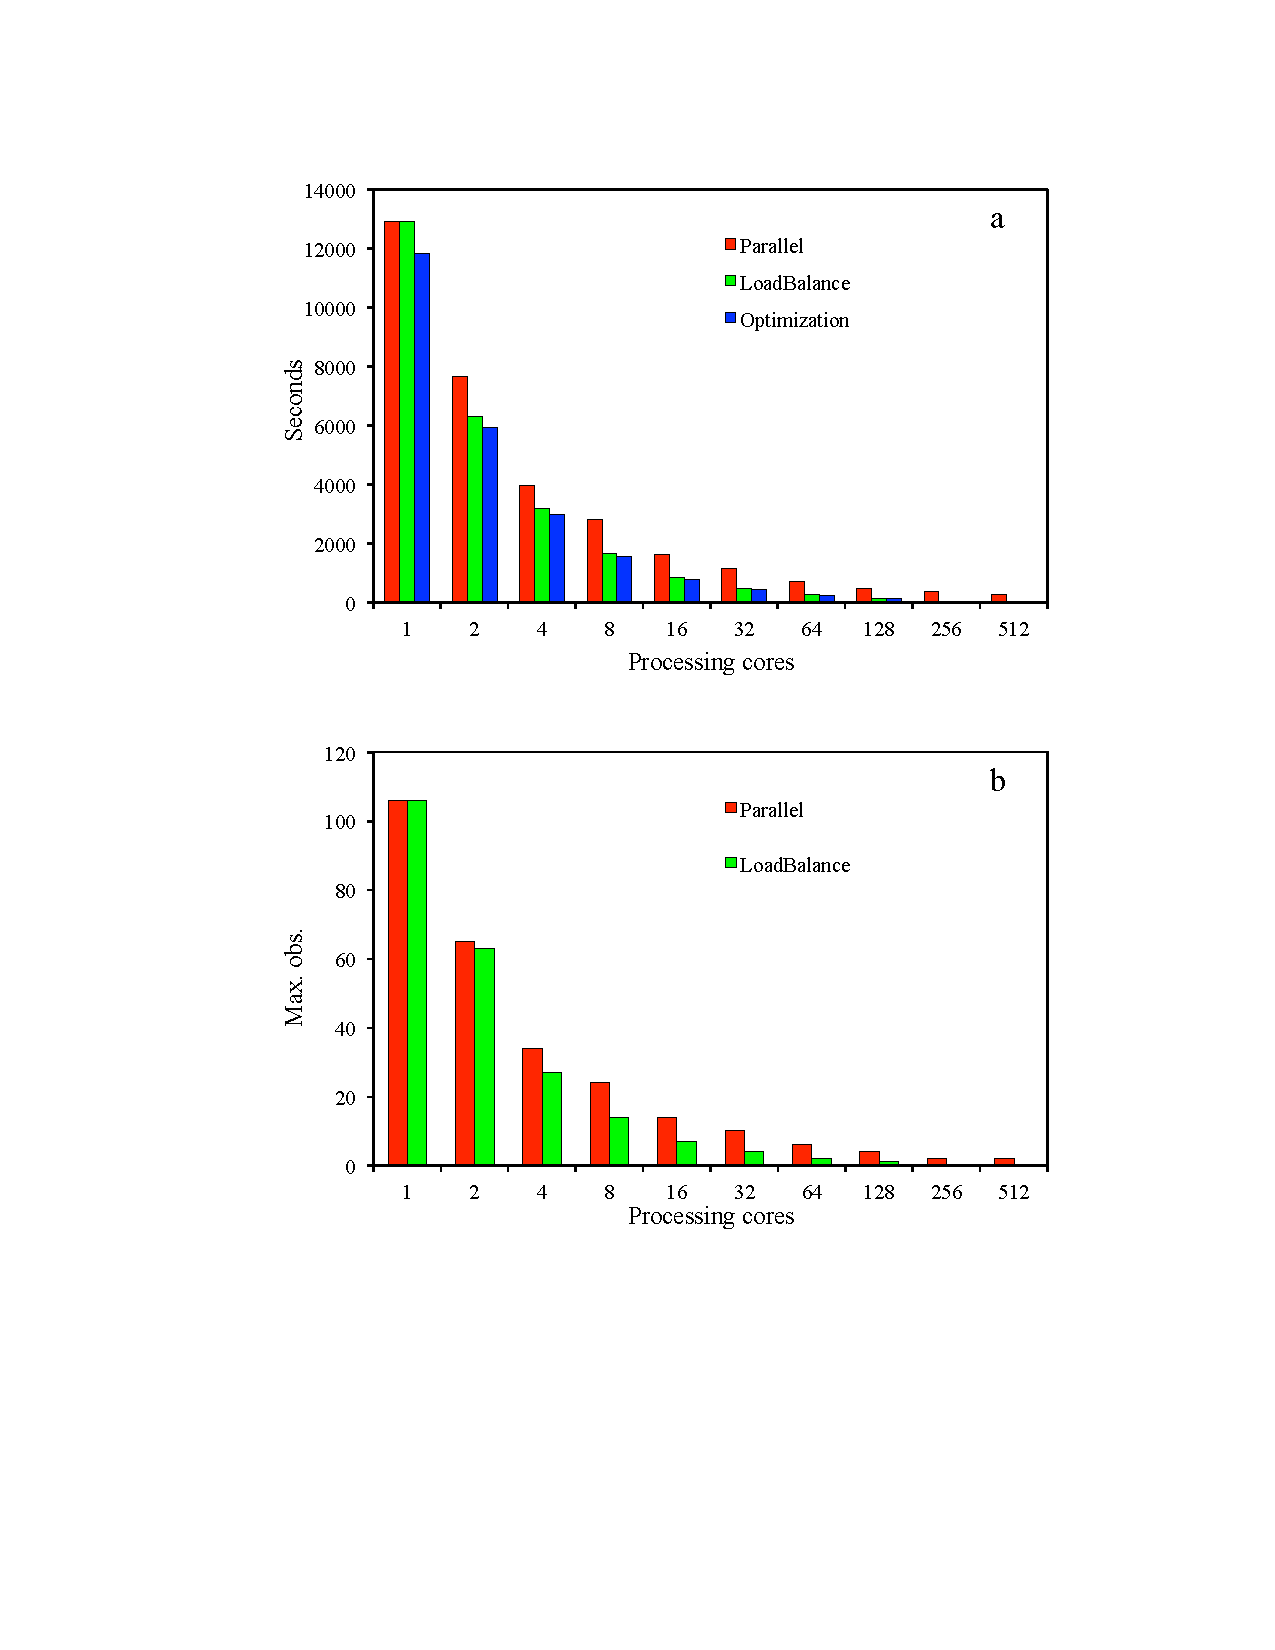
\includegraphics[width=40pc, trim=30 200 100 50, clip]{figures/Walltime.pdf}
\caption{The wallclock times (a) and maximum number of observation per processing core (b) for 5 iterations of minimization on NCAR yellowstone.}
\label{timing}
\end{figure}
%
\begin{figure}
\noindent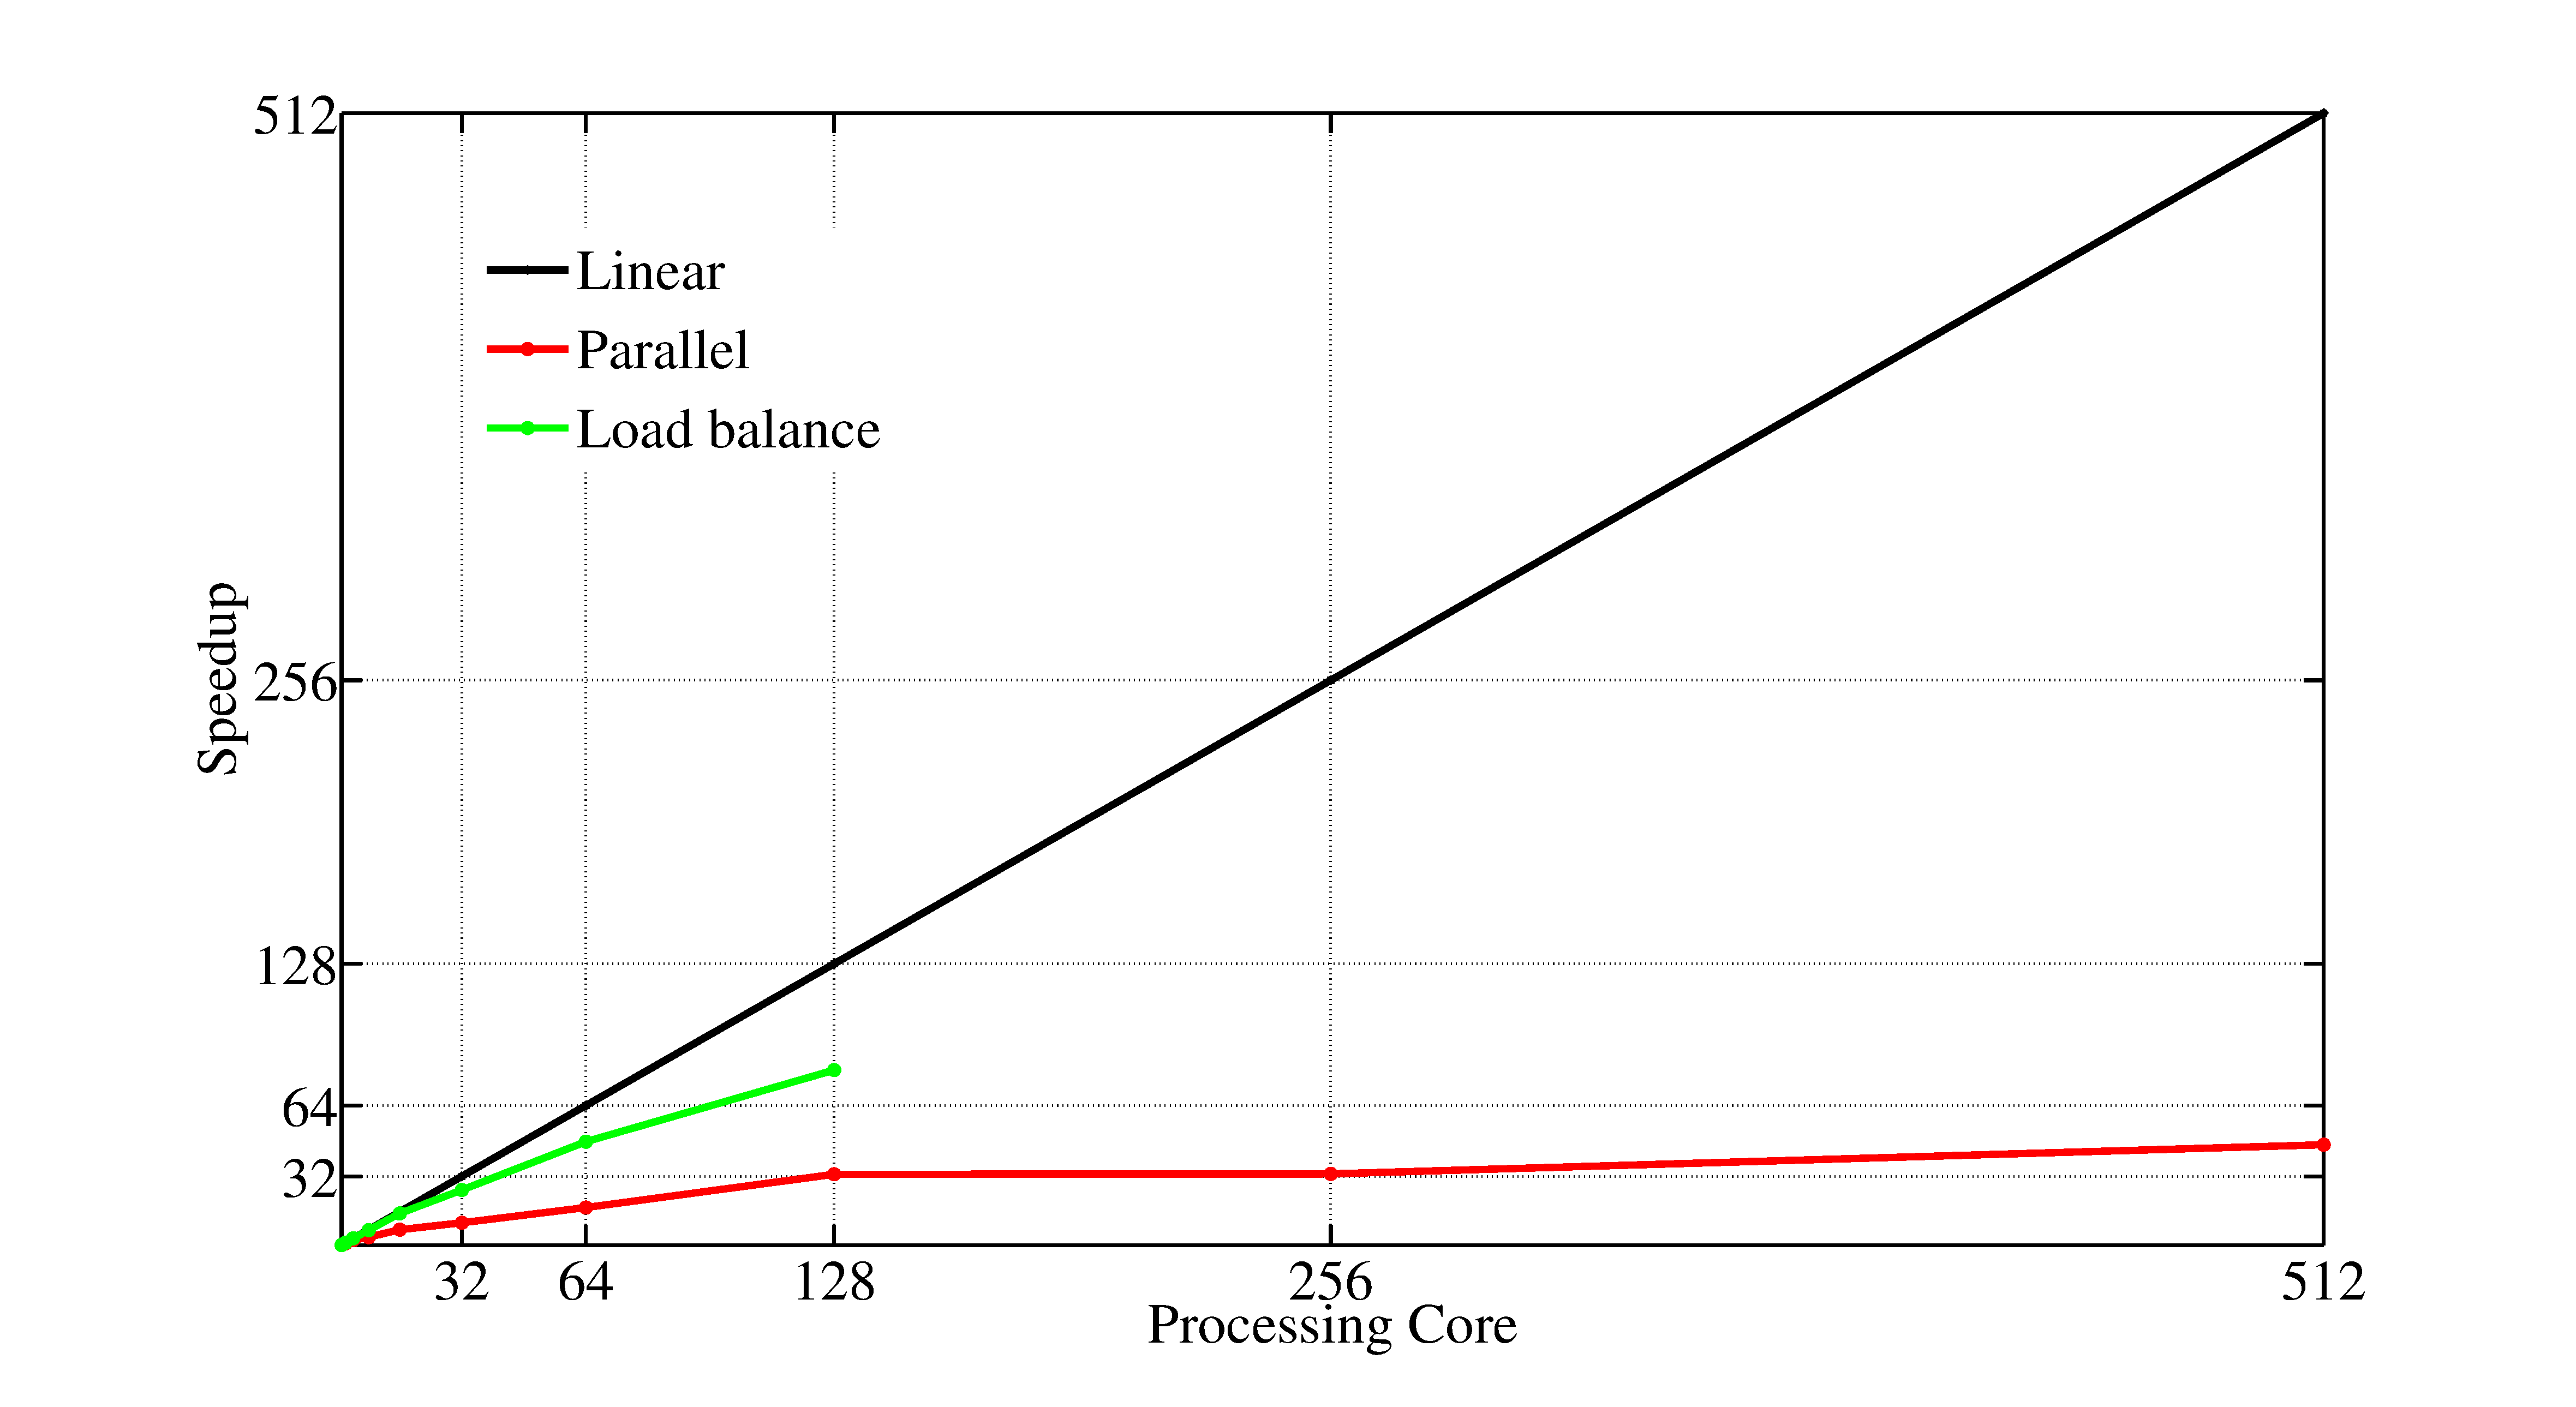
\includegraphics[width=40pc,trim=30 20 150 50, clip,]{figures/speedup.eps}
\caption{The same as Fig. \ref{timing} ,but for the parallel speedup}
\label{spd}
\end{figure}
%
% ---------------
% EXAMPLE TABLE
%
%\begin{table}
%\caption{Time of the Transition Between Phase 1 and Phase 2\tablenotemark{a}}
%\centering
%\begin{tabular}{l c}
%\hline
% Run  & Time (min)  \\
%\hline
%  $l1$  & 260   \\
%  $l2$  & 300   \\
%  $l3$  & 340   \\
%  $h1$  & 270   \\
%  $h2$  & 250   \\
%  $h3$  & 380   \\
%  $r1$  & 370   \\
%  $r2$  & 390   \\
%\hline
%\end{tabular}
%\tablenotetext{a}{Footnote text here.}
%\end{table}

% See below for how to make sideways figures or tables.

\end{document}

%%%%%%%%%%%%%%%%%%%%%%%%%%%%%%%%%%%%%%%%%%%%%%%%%%%%%%%%%%%%%%%

More Information and Advice:

%% ------------------------------------------------------------------------ %%
%
%  SECTION HEADS
%
%% ------------------------------------------------------------------------ %%

% Capitalize the first letter of each word (except for
% prepositions, conjunctions, and articles that are
% three or fewer letters).

% AGU follows standard outline style; therefore, there cannot be a section 1 without
% a section 2, or a section 2.3.1 without a section 2.3.2.
% Please make sure your section numbers are balanced.
% ---------------
% Level 1 head
%
% Use the \section{} command to identify level 1 heads;
% type the appropriate head wording between the curly
% brackets, as shown below.
%
%An example:
%\section{Level 1 Head: Introduction}
%
% ---------------
% Level 2 head
%
% Use the \subsection{} command to identify level 2 heads.
%An example:
%\subsection{Level 2 Head}
%
% ---------------
% Level 3 head
%
% Use the \subsubsection{} command to identify level 3 heads
%An example:
%\subsubsection{Level 3 Head}
%
%---------------
% Level 4 head
%
% Use the \subsubsubsection{} command to identify level 3 heads
% An example:
%\subsubsubsection{Level 4 Head} An example.
%
%% ------------------------------------------------------------------------ %%
%
%  IN-TEXT LISTS
%
%% ------------------------------------------------------------------------ %%
%
% Do not use bulleted lists; enumerated lists are okay.
% \begin{enumerate}
% \item
% \item
% \item
% \end{enumerate}
%
%% ------------------------------------------------------------------------ %%
%
%  EQUATIONS
%
%% ------------------------------------------------------------------------ %%

% Single-line equations are centered.
% Equation arrays will appear left-aligned.

Math coded inside display math mode \[ ...\]
 will not be numbered, e.g.,:
 \[ x^2=y^2 + z^2\]

 Math coded inside \begin{equation} and \end{equation} will
 be automatically numbered, e.g.,:
 \begin{equation}
 x^2=y^2 + z^2
 \end{equation}

% IF YOU HAVE MULTI-LINE EQUATIONS, PLEASE
% BREAK THE EQUATIONS INTO TWO OR MORE LINES
% OF SINGLE COLUMN WIDTH (20 pc, 8.3 cm)
% using double backslashes (\\).

% To create multiline equations, use the
% \begin{eqnarray} and \end{eqnarray} environment
% as demonstrated below.
\begin{eqnarray}
  x_{1} & = & (x - x_{0}) \cos \Theta \nonumber \\
        && + (y - y_{0}) \sin \Theta  \nonumber \\
  y_{1} & = & -(x - x_{0}) \sin \Theta \nonumber \\
        && + (y - y_{0}) \cos \Theta.
\end{eqnarray}

%If you don't want an equation number, use the star form:
%\begin{eqnarray*}...\end{eqnarray*}

% Break each line at a sign of operation
% (+, -, etc.) if possible, with the sign of operation
% on the new line.

% Indent second and subsequent lines to align with
% the first character following the equal sign on the
% first line.

% Use an \hspace{} command to insert horizontal space
% into your equation if necessary. Place an appropriate
% unit of measure between the curly braces, e.g.
% \hspace{1in}; you may have to experiment to achieve
% the correct amount of space.


%% ------------------------------------------------------------------------ %%
%
%  EQUATION NUMBERING: COUNTER
%
%% ------------------------------------------------------------------------ %%

% You may change equation numbering by resetting
% the equation counter or by explicitly numbering
% an equation.

% To explicitly number an equation, type \eqnum{}
% (with the desired number between the brackets)
% after the \begin{equation} or \begin{eqnarray}
% command.  The \eqnum{} command will affect only
% the equation it appears with; LaTeX will number
% any equations appearing later in the manuscript
% according to the equation counter.
%

% If you have a multiline equation that needs only
% one equation number, use a \nonumber command in
% front of the double backslashes (\\) as shown in
% the multiline equation above.

%% ------------------------------------------------------------------------ %%
%
%  SIDEWAYS FIGURE AND TABLE EXAMPLES
%
%% ------------------------------------------------------------------------ %%
%
% For tables and figures, add \usepackage{rotating} to the paper and add the rotating.sty file to the folder.
% AGU prefers the use of {sidewaystable} over {landscapetable} as it causes fewer problems.
%
% \begin{sidewaysfigure}
% \includegraphics[width=20pc]{samplefigure.eps}
% \caption{caption here}
% \label{label_here}
% \end{sidewaysfigure}
%
%
%
% \begin{sidewaystable}
% \caption{}
% \begin{tabular}
% Table layout here.
% \end{tabular}
% \end{sidewaystable}
%
%

